\documentclass[a3paper,12pt]{article}
\usepackage[utf8]{inputenc}
\usepackage[english]{babel}
\usepackage{tikz-cd}
\usepackage{amsmath,amsfonts,amssymb,amsthm}
\usepackage{mathtools}
 \usepackage{float}
\usepackage{amsthm}
\usepackage{cite}
\usepackage{datetime} % British format dates
\usepackage[cm]{fullpage}
\usepackage{url}
\usepackage{hyperref}
\usepackage{stackrel,amssymb,amsmath}
\usepackage[nottoc]{tocbibind}
\usepackage{rotating}
\usepackage[autostyle]{csquotes}
\usepackage{natbib}
\usepackage{graphicx}
%\usepackage{natbib}
\usepackage{graphicx}
\usepackage{tikz}
\usetikzlibrary{arrows}

\newtheorem{problem}{Problem}
\newtheorem{attempt}{Attempt}
\newtheorem{theorem}{Theorem}[section]
\newtheorem{corollary}{Corollary}[theorem]
\newtheorem{lemma}[theorem]{Lemma}
\newtheorem{proposition}[theorem]{Proposition}
\theoremstyle{definition}
\newtheorem{definition}{Definition}[section]
%\theoremstyle{indented}
\newtheorem*{remark}{Remark}
\newenvironment{titlemize}[1]{%
  \paragraph{#1}
  \begin{itemize}}
  {\end{itemize}}
  
\theoremstyle{definition}
\newtheorem{example}{Example}[section]  
\theoremstyle{definition}
\newtheorem{exercise}{Exercise}[section]  



\title{Combinatorics of $\tilde{P}_n$}
\author{Rhys Wells}
\date{\today}

\begin{document}

\maketitle
\tableofcontents

\section{Introduction and motivation}

We want to generalise the geometric stability conditions $\sigma_{\phi}(G)$ to combinatoric stability condition denoted as $\sigma(G)$. To do so we abstract out two key characteristics of $\sigma_{\phi}(G)$: that the sets $\sigma_{\phi}(G)$ induces a free transitive action of $J(G)$, and elements of $\sigma_{\phi}(G)$ are near each other.\\

The combinatorics of this set up are discussed in \cite[Section 3.5]{caporaso2019combinatorics}.

% The combinatorics of compactified jacobians are discussed in \cite[Section 3.3]{caporaso2019combinatorics}.


\section{Notation}

Let $X$ be a curve and $G$ be its dual graph where $G=(V,E)$ is a vertex labelled multigraph. Let $\Gamma$ a spanning tree of the graph $G$ (a subtree of $G$ that contains all vertices of $G$) and let $I$ be the index set for the spanning trees of $G$.  The first betti number of a graph $b_1(G)=|E|-|V|+1$ is the number of independent loops, and note that $b_{1}(G) = \#Edges(G\setminus \Gamma)$. \\ %b1(G)=(rank of the first homology group). \\

Throughout these notes we consider only single curve stability conditions for line bundles.

\section{Geometric stability conditions}

% In this case the data of the sheaf relies only on discrete data specifically the muiltdegree of $F$ and the locus where its not locally free (subsets of the nodes).

For a single curve with the associated graph $G$ we consider the total degree $0$ stability space,
$$V(G)=\{d : \text{Vert}(G) \rightarrow \mathbb{R} \mid \sum_{v \in \text{Vert}(G)} d(v) =0 \} \subseteq \mathbb{R}^{\text{Vert}(G)}$$
with integer lattice points given by 
$$S(G) = \{d : \text{Vert}(G) \rightarrow \mathbb{Z} \mid \sum_{v \in \text{Vert}(G)} d(v) =0 \} \subseteq \mathbb{Z}^{\text{Vert}(G)}$$ 

where $S(G)\subseteq V(G)$. One can define stability polytopes $P$ as connected components of the complement of $V(G)$ with stability hyperplanes (see \cite[Definition 5.1]{kass2019stability}), we denote the set of polytopes as $Q_G$. The integer lattice points of these polytopes are given as follows where for line bundles the following relation is deduced from \cite[Definition 2.5]{pagani2020geometry}.

\begin{definition}\label{linebundleinequal}
Let $\phi \in V(G)$, we say $d \in S(G)$ is $\phi$-(semi) stable if,

\begin{equation}\label{stabinequal}
\Bigl| \sum_{v \in Vert(G_0)} d(v) - \phi(v)\Bigr| \underset{(\le)}{<}  \frac{\# (E(G\setminus G_0) \cap E(G\setminus G_0^{c}) )}{2},
\end{equation}

for all $\emptyset \subsetneq G_0 \subsetneq G $, where $G_0$ is a complete subgraph ($G_0^{c}$ denotes the complete subgraph with complement vertices to $G_0$).
\end{definition}

\begin{remark}
 The complete graph $G_0$ is determined by the choice of vertices (partitioning Vert($G$) into disjoint sets). The term $\# (E(G\setminus G_0) \cap E(G\setminus G_0^{c}) )$ denotes the number of edges given by a cut of $G$.
\end{remark}

Let $\phi\in V(G)$ and take $\phi$ to be non-degenerate that is if $\phi\in P$ for some $P \in Q_G$, or equivalently for all $d$ equation (\ref{stabinequal}) is a strict inequality.

\begin{definition} The set of geometric stability conditions is given by,
$$\sigma_{\phi}(G):=\{d : \text{Vert}(G) \rightarrow \mathbb{Z} \mid \phi \text{-stable}\} \subseteq S(G).$$
\end{definition}

\begin{example}

We will now $\phi$-stability Vine Curves. Vine curves have graphs $G$ with two vertices and $k$ edges. This example is from \cite[Example 3.18]{Kass_2017}. Let $G_0$ be a single vertex, then ${\# (E(G \setminus G_0) \cap E(G \setminus G_0^{c}) )}=k.$ Let $\phi \in V(G)$ and $d\in S(G)$, without lose of generality let $d=(d_1,-d_1) $ so its enough to consider only $d_1 \in \mathbb{Z}$. In particular if $\phi$ is non-degenerate we have the Oda-inequaliy,

\begin{equation}\label{vineOda}
|d_1-\phi_1|<\frac{k}{2}.
\end{equation}

Equation (\ref{vineOda}) requires us to take $d$ to be the $k$ closest integers to $\phi$. We aim to find which $\phi \in V(G)$, is a given set of $d$, $\phi$-stable i.e. to determine $\sigma_{\phi}(G)$. If $k$ is even then $\phi$ is non-degenerate if and only if $\phi \notin \mathbb{Z}$. If $k$ is odd $\phi$ is non-degenerate if and only if $\phi \in \frac{1}{2}+\mathbb{Z}$. Let $k=2$ and $\phi=(\frac{1}{2},-\frac{1}{2})$ then 

$$\sigma_{\phi}(G) =\{(0,0),(1,-1)\}.$$
\end{example}


\begin{example}

We will now discuss the $\phi$-stability of Necklace Curves. Necklace curves are denoted as $I_n$ with $n$ components, for a fixed $I_n$ let $G$ be the associated graph. We have $ {\# (E(G \setminus G_0) \cap E(G \setminus G_0^{c}) )}=1$ as each cut for a necklace curve gives $2$ edges. Let $\phi \in V(G)$, the $\phi$-(semi)stable multidegrees for a necklace curve are given by the set,
$$ \sigma_{\phi}(G) = \left\{ d\in S(G) \text{ s.t } \Bigl|{\sum_{i \in I_0} d_i - \phi_i \Bigr| \le 1,\: \forall \: \emptyset \subsetneq I_0 \subsetneq I\right\} \subseteq S(G)$$
where each $I_0$ is a consecutive set. Consider the graph from example \ref{triangle} and let $\phi=(\frac{1}{3},\frac{1}{3},-\frac{2}{3})$ we have,

$$\sigma_{\phi_1} (G)=\{(0,0,0), (1,0,-1), (0,1,-1)\}.$$

Similarly if $\phi_2=(-\frac{1}{3},-\frac{1}{3},\frac{2}{3})$, then $\sigma_{\phi_2} (G)=\{(0,0,0), (-1,0,1), (0,-1,1)\}$.


\end{example}

\begin{example}

Consider the graph of example \ref{noAutTrans}. We have $Aut(G)=\mathbb{Z}/2\mathbb{Z}$ and $J(G)=\mathbb{Z}/5\mathbb{Z}$. If we let $\phi=(\frac{1}{3},\frac{1}{3},-\frac{2}{3})$ we have the inequalities 

$$|d_1-\phi_1| \le \frac{3}{2},|d_2-\phi_2| \le 1,|d_3-\phi_3| \le \frac{3}{2}$$

and so $\sigma_{\phi}(G)=\{(0,0,0),(-1,0,1),(1,0,-1),(1,-1,0),(0,-1,1)\}.$

% If we take the average of $d \in \sigma(G)$ we get $(\frac{1}{5},-\frac{2}{5},\frac{1}{5})$.

\end{example}


\section{Combinatoric stability conditions}

In this section we introduce the notions to understand a generalisation of geometric stability conditions and give the definitions, as well as state future problems of interest. Generalise stability conditions for single curves in $g=1$ are discussed in \cite[Definition 6.5]{pagani2020geometry}.

\subsection{Construction of $J(G)$}

To introduce generalised stability conditions we need enter the realm of algebraic graph theory to discuss the Jacobian of a graph, which is derived from the study of the chip-firing action on divisors $Div(G)\cong \mathbb{Z}^{Vert(G)}$ on $G$, see \cite[Chapter 2]{corry2018divisors}. For $D , D^{'} \in Div(G)$ one fires from a vertex $v$ on $D$ to obtain $D^{'}$ by mapping $D$ to 

$$D^{'}= D - deg(v)+\sum_{vw\in E} w.$$

We see the number of chips fired from a vertex is equal to the sum of chips received from the corresponding vertices, therefore the total degree remains constant after applying firing scripts. One can also similarly define the reverse mapping. Sets of vertices can be fired multiple times at once and are called firing scripts where the set of all firing scripts is denoted by $\mathbb{Z}^{Vert(G)}$. Divisors $D$ and $D^{'}$ are linearly equivalent if $D-D^{'}=div(f)$ for a firing script $f$. To a firing script we can associate a divisor as follows.

\begin{definition}
Consider the linear map $div: \mathbb{Z}^{\text{Vert}(G)} \rightarrow \mathbb{Z}^{\text{Vert}(G)}$ and let $f \in \mathbb{Z}^{\text{Vert}(G)}$ where

\begin{equation}
    div(f)= \sum_{v \in \text{Vert}(G)} \left( deg(v)\cdot f(v) - \sum_{vw \in E(G)} f(w) \right) \cdot v
\end{equation}
\end{definition}
In particular $div(\mathbb{Z}^{Vert(G)})$ often called $Prin(G)$ is a subset of $S(G)$ (in firing chips the total money of system stays constant) additionally $div$ is a homomorphism of $\mathbb{Z}$-modules. %(abelian groups).
The cokernal of the div map defines $Pic(G)$. As our graph is labelled so we can identify the div map with the discrete Laplacian \cite[Section 2.1]{corry2018divisors}, which can be used to explicitly calculate $Pic(G)$ and more importantly $J(G)$. Let $Deg$ be the valency matrix and Adj be the adjacency matrix. The discrete Laplacian is given as $L: \mathbb{Z}^{Vert(G)} \rightarrow \mathbb{Z}^{Vert(G)}$ such that 
$$L=Deg-Adj^{T}.$$
Similar to $Pic(G)$ the group $J(G)$ is defined using the reduced $div$ map and is determined by deleting the row and column of $L$ corresponding to a chosen sink ($J(G)$ can be shown to be independent of this choice). Another way to view $J(G)$ is by considering the following induced group action on $S(G)$,
\begin{align*}
    \alpha: \mathbb{Z}^{Vert(G)} \times S(G) &\rightarrow S(G)\\
    (f,d) & \mapsto div(f)+d
\end{align*}

 and so one can consider the set of orbits $J(G):=S(G)/ div(\mathbb{Z}^{Vert(G)} ) $ with the quotient map
$$\pi: S(G) \rightarrow J(G). $$

As $S(G)$ is an abelian group so $J(G)$ is a group, as all subgroups of abelian group are normal and as $div(\mathbb{Z}^{Vert(G)})$ is finite index subgroup of $S(G)$ by the first isomorphism theorem. By studying the invariant factors of the reduced Laplacian the order of $J(G)=det(\tilde{L})$ and by Kirchhoff’s Matrix-Tree Theorem \cite[Section 9.1]{corry2018divisors}, $J(G)$ is a finite abelian group whose order is the number of spanning trees in $G$ (complexity of $G$). 

\begin{example}\label{triangle}

Consider the following graph,
\begin{center}
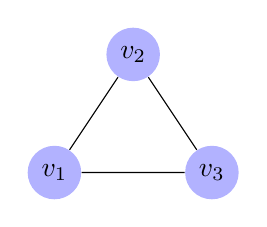
\begin{tikzpicture}[main_node/.style={circle,fill=blue!30,minimum size=1em,inner sep=3pt]}]

    \node[main_node] (1) at (0,0) {$v_2$};
    \node[main_node] (2) at (-1, -1.5)  {$v_1$};
    \node[main_node] (3) at (1, -1.5) {$v_3$};

    \draw (1) -- (2) -- (3) -- (1);
\end{tikzpicture}
\end{center}

with the Laplacian,

$$L=
\begin{pmatrix}
2 & -1 & -1\\
-1 & 2 & -1\\
-1& -1& 2
\end{pmatrix}
$$

and $J(G)=\mathbb{Z}_3.$ 
\end{example}

\begin{example}\label{noAutTrans}

We see that the graph,

\begin{center}
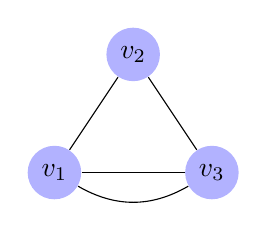
\begin{tikzpicture}[main_node/.style={circle,fill=blue!30,minimum size=1em,inner sep=3pt]}]

    \node[main_node] (1) at (0,0) {$v_2$};
    \node[main_node] (2) at (-1, -1.5)  {$v_1$};
    \node[main_node] (3) at (1, -1.5) {$v_3$};
    
  \path[every node/.style={font=\sffamily\small}]
    (1) edge node [] {} (2)
    % (1) edge[bend left] node [] {} (2)
    (2) edge node [] {} (3)
    (3) edge node [] {} (1)
    (3) edge[bend left] node [] {} (2);

    % (3) edge[bend right] node [left] {} (2);

\end{tikzpicture}
\end{center}

has the Laplacian 

$$ L=
\begin{pmatrix}
3 & -1 & -2\\
-1 & 2 & -1\\
-2& -1& 3 
\end{pmatrix}
$$

and $Jac(G)=\mathbb{Z}_5$ and $Aut(G)=\mathbb{Z}_2$.
\end{example}



%And by \cite[Theorem 1.13]{sampayne665} the absolute value of the determinant of the reduced graph Laplacian of a graph G is equal to the number of spanning trees in
% $G$.

% \item By the theorem of finitely generated abelian groups $J(G)$ has invariant factors.

\subsection{Complete set of representatives for the $J(G)$ action}

The group $J(G)$ acts on $\sigma_{\phi}(G)$ by translation \cite[Lemma 3.25,p.19]{Kass_2017} freely and transitively. The set $\sigma_G(\phi)$ is a full set of representatives for the action of $J(G)$ (Is this true, is there a reference?)\\

Let $\sigma(G)$ be a complete set of representatives for the action of $J(G)$ on $S(G)$. Therefore for all $c \in S(G)$ there exists a unique $d \in \sigma(G) $ such that, $c=div(f)+d \in S(G)$ and equivalently $c-d \in div(\mathbb{Z}^{Vert(G)})$. This is equivalent to $\sigma(G)$ being a section of the quotient map $\pi: S(G) \rightarrow J(G)$ (see \cite[Abstract]{AN_2014}). As $\sigma(G)$ is a complete set of representatives so it admits a action by translating by elements of $J(G)$ \cite[p.55]{corry2018divisors}, which additionally is free and transitive. Let $e \in S(G)$ such that $\pi(e)=g$ then we have the following action,
\begin{align*}
    \beta: Jac(G) \times \sigma(G) &\rightarrow S(G)\\
    (g,d) & \mapsto \text{The unique element of $\sigma(G)$ that represents $e+d$ }.
\end{align*}

To check this action is well defined let $\pi(e)=\pi(e^{'})=g$, then as $\pi$ is a homomorphism so $\pi(e)-\pi(e^{'})=\pi(e-e^{'})=0$ and as $div(\mathbb{Z}^{Vert(G)}) = \pi^{-1}([0])$ so 

$$\beta(g,d)-\beta(g,d) =e+d-e^{'}+d=e-e^{'} \in div(\mathbb{Z}^{Vert(G)}).$$

\begin{remark}
 By the free transitive $J(G)$ action we have $|\sigma(G)|=|J(G)|=|\#\text{Spanning trees}|$ and so $\sigma(G)$ is finite. Additionally as $\beta$ is a free transitive action so each $\sigma(G)$ is a principal homogeneous $Jac(G)$-space.\\ %Related to principal bundles & torsors. A free and transitive action is equivalent to a simply transitive action.
\end{remark}

The sets $\sigma(G)$ are "good choices" for identity elements of $J(G)$, in that $Pic^{d}(G)$ is a torsor of $Jac(G)$ (see \cite[p.55]{corry2018divisors}). Choosing an element of $\sigma(G)$ is equivalent to giving a bijection of sets $\phi: \sigma(G) \rightarrow J(G)$. To show this consider a bijection $\phi$ and let $\phi^{-1}([0]) \in \sigma(G)$, and note $\sigma(G)$ is a complete set of representatives. Inversely let $a \in \sigma(G)$ and $d \in S(G)$ define the mapping $\phi_a(d)=[d-a]$ (see \cite[Proposition 2.12]{corry2018divisors}). 


% \begin{remark}
% We fix an element of $\sigma(G)$ to act as the origin of $J(G)$.\\
% \end{remark}

\begin{remark}
Not all complete sets of representative are of the form $\sigma_{\phi}(G)$. For example critical, superstable and break configurations are all class representatives of $J(G)$ of see \cite[Proposition 4.7.6]{klivans2018mathematics}. To generalise $\sigma_{\phi}(G)$ properly we need to add an extra axiom to include the notion of nearness. 
\end{remark}

\begin{example}
Consider the vine graph with $k=2$ edges. The div map sends $(1,0) \mapsto (-2,2)$ and $(0,1) \mapsto (2,-2)$. For $(d,-d) \in \mathbb{Z}^{2}$ one has $div((d,-d)) = (d-2,d+2)$ so if $d$ is odd it remains odd, similarly if it is even then it remains even. The following set 
$$\sigma(G) =\{(1,-1),(4,-4)\}$$
is a complete class of representatives for $J(G)$. But the set $\sigma(G) =\{(1,-1),(3,-3)\}$ is not, as acting by $J(G)$ we only get $(d,-d)$ with $d$ odd. Neither sets, will be seen to satisfy axiom 2 (nearness) as in the $\sigma_{\phi(G)$ case.
\end{example}

\subsection{Generalised stability conditions}

Recall the definition of a integral break divisors, IBD, from \cite{AN_2014}. These are constructed by taking all spanning trees and adding $1$ at the endpoints in all possible ways. For example consider the graph of example \ref{noAutTrans} we take the following IBD these are distinct divisors for all trees with $deg(D)=b_1(G)=g$, 
% There are many class reps but they are dependant on their construction/ procedure.

$$\{(2,0,0), (1,0,1), (0,0,2), (1,1,0) , (0,1,1)\}.$$

In particular IBD are a class of representatives for the $J(G)$ action. To defined a generalised stability condition and in order to remain in the total degree $0$ stability space after adding IBD, we consider the following set of divisors

$$S^{-b_{1}(G)}(G)=\{d^{'} \in \mathbb{Z}^{Vert(G)} \mid \sum d^{'}(v) = -b_{1}(G)\}.$$

And denote the set of orientations of $G \setminus \Gamma$ to be $S=\{s:Edges(G \setminus \Gamma) \rightarrow Vert(G)$\} and denote the set of divisors near $d^{'} \in S^{-b_{1}(G)}(G)$ to be,

$$\sigma^{'}(\Gamma,d^{'}
):= \{ d \in S(G) \mid d= d^{'} + \sum_{l \in E(G\setminus \Gamma)} \delta _{s(l)} \text{ for } s \in S  \}.$$

\begin{definition}\label{axioms12}
A generalised stability condition for $G$ is a subset $\sigma(G) \subseteq S(G)$ such that,

\begin{enumerate}
    \item the set $\sigma(G)$ is a complete set of representatives for the action of $J(G)$
    
\item and for each spanning tree $\Gamma_i$ for $i \in I$, there exists $d_i^{'} \in S^{-g}$ such that 

$$\sigma(G) = \bigcup_{i\in I} \sigma^{'}(\Gamma_i,d_{i}^{'}).$$

\end{enumerate}
\end{definition}

\begin{remark}
 Axiom 1 is from the fact the $\overline{J}$ is proper. And axiom 1 is from that $\overline{J}$ is open. 
\end{remark}

\begin{remark}
Axiom 2 can be thought of as adding chips at the endpoints of $G\setminus \Gamma$ in all possible ways. Axiom 2 is discussed in \cite[5.12]{christ2019compactified}, \cite{Nic2017MO} and \cite[Def 8.5.1]{klivans2018mathematics}. Generalised stability conditions may be called generalised break divisors as in \cite[Theorem 3.5]{yuenMatriodsgeometric} or integral break divisors as in \cite[4.4]{AN_2014}. The definition of $\sigma(G)$ appears to be related to the Bernardi torsor action see \cite[p.121]{klivans2018mathematics}. 
\end{remark}

\begin{remark}
In $g=1$ a generalised stability is called an assignment \cite[Definition 6.8]{pagani2020geometry}. In this case \cite[Corollary 2.15 and 3.12]{pagani2020geometry} constitute axioms $1$ and $2$. To see this notation in $g=1$ case See \cite[Notation 3.5, (3)]{pagani2020geometry} and \cite[Lemma 3.6]{pagani2020geometry}.
\end{remark}

\begin{example}
We will now describe $\sigma(G)$ for graphs of vine curves. From the Laplacian the Jacobian can be easily calculated. For vine curves with $k$ edges we have $J(G)=\mathbb{Z}_k$. Note the spanning trees are identical for vine curves. For $d^{'} \in N$ we have ${d}^{'} = (d^{'}, -k+1-d^{'})$ and  
$$\sigma^{'}(\Gamma,d^{'}) = \{(d^{'}+k-1,-k+1-d^{'}) , \dots ,(d^{'},-d^{'})\}$$
By axiom $1$ we have $|\sigma(G)|=|J(G)|=k$ so 

$$\sigma(G) = \{(d^{'}+k-1,-k+1-d^{'}) , \dots ,(d^{'},-d^{'})\}.$$

% In the case where $k=2$. Consider $d^{'} \in N$ these are $(d^{'},-1-d^{'})$ with $\sigma^{'}(\Gamma,d^{'}) = \{(d^{'}+1,-1-d^{'}) , (d^{'},-d^{'})\}$. 

% $$\sigma(G)=\left\{ (d,-d), (d+1,-d-1),\dots,(d+k-1,-d-k+1) \right\}.$$

\end{example}
\begin{remark}
Not all elements of $\sigma_G$ have a nice form as in the vine curve case. 
\end{remark}
\begin{example}
We will now describe $\sigma(G)$ for the necklace curves. Consider the graph of $I_n$ and let $d^{'} \in N$ and consider a spanning tree $\Gamma $. Then elements of $\sigma(G)$ are zero of all elements expect on one vertex where it has value $1$ and a different vertex where it has value $-1$ (as asked in \cite{Nic2017MO}).

\end{example}

\subsection{Does there exist a $\phi$ for a generalised stability condition?}

\begin{definition} Denote the set of all generalised stability conditions by,
$$\Sigma_{G} = \left\{ \sigma(G) \subseteq S(G) \mid \sigma(G) \text{ is a generalised stability condition} \right\}\subseteq 2^{S(G)}$$

\end{definition}



\begin{theorem}
The map, 
\begin{align*}
    \psi_G: Q_G &\rightarrow \Sigma_G\\
    \phi \in P &\mapsto \sigma_{\phi}(G) 
\end{align*}

is injective

\end{theorem}

\begin{proof}
See Nicolas talk in roam classifying FCUJ.

\cite[Lemma 3.3.2]{caporaso2019combinatorics}

\end{proof}



\begin{titlemize}{Objective}
\item Try to fix a procedure to show $\psi_G$ is surjective, that is for all $\sigma \in \Sigma_G$ there exist a nondegenerate $\phi \in V(G)$, such that $\sigma_{\phi}(G)=\sigma(G)$ for arbitrary graphs.

\item Or disprove this result by finding a suitable graph (non-planer).

\item To approach this move to isomorphism classes with $b_1(G)=2$ next. If $G$ has a separating edge (an $E$ such that $G \setminus E=G_1 \cup G_2$) we can reduce the problem to considering the conjecture on $G_1$. For an idea see ABKS Decomposition in \cite[Figure 1]{AN_2014}.
\end{titlemize}

\subsection{From seminar classifying FCUJ}



\subsection{If $Aut(G)$ acts transitively then take the average}

An element $\alpha \in Aut(G)$ maps pair of vertices $(u,v)$ form an edge if and only if the pair $(\alpha(u),\alpha(v))$ also form an edge.\\

Nicolas thinks if $Aut(G)$ acts transitively on $G$ (acts transitively on $Vert(G)$ i.e vertex transitive graph, which implies it is a regular graph) then taking the average might still work to find a $\phi$ such that $\sigma_{\phi}(G)=\sigma(G)$, as $Aut(G)$ "fixes" the oda inequalities. For the necklace case this is seen in \cite[Proposition 7.4]{melo2015fine}.\\


%By this reference consider, how the chamber for $\sigma_{\phi}(G)$ is defined. Starting from $\sigma(G)$ (complete set of representations) want to define a $\phi$, how are $\phi$ defined (just elements of $\mathbb{R}^{n}$ that sits inside Oda inequalities for those $d$ for subcurves). How are the subgraphs of $G$ defined.

We see $\sigma(G)$ as torsors, and in \cite[Definition 3.24]{corry2018divisors} it discusses averaging and harmonic functions.



\printindex

\bibliographystyle{alpha}
\bibliography{bibtex}

\end{document}